\chapter{Hexagonales Schach}

Hexagonales Schach hat viele unterschiedliche Spielweisen. Diese variieren nicht nur in den möglichen Zügen, sondern auch der Anzahl der Spielsteine und der Größe des Spielfelds. Glinskis Regeln werden für die Europameisterschaften in hexagonales Schach genutzt \cite{Gados:Hexagonal}. In der Version von Glinski besteht das Spielbrett aus 91 Feldern. Da jede Seite gleichlang ist, ist das Feld ein perfektes Hexagon. Dies ist nicht in jeder Schachvariante gleich. Schafran lässt die Spalten a und l aus (vgl. Abbildung \ref{fig:hex:start}). Dazu variiert noch die Startaufstellung.

\begin{figure}[H]
    \centering
    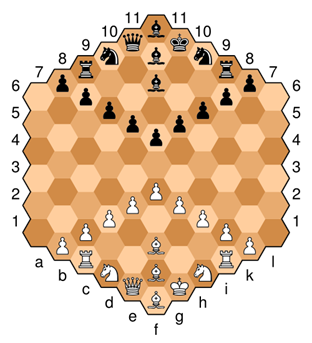
\includegraphics{images/hexStart.png}
    \caption{Startaufstellung Glinski \protect\footnotemark}
    \label{fig:hex:start}
\end{figure}
\footnotetext{\url{https://commons.wikimedia.org/wiki/Category:Glinski\%27s_hexagonal_chess}}

\begin{table}[H]
    \centering
    \begin{tabular}{|c|c|}
        \hline
        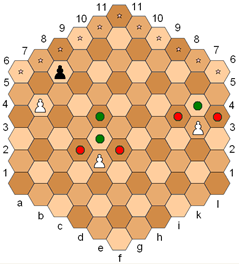
\includegraphics{images/hexPawn.png} & 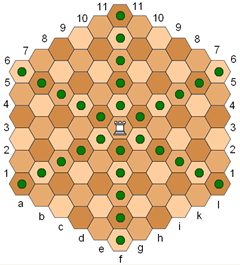
\includegraphics{images/hexRook.png} \\ \hline 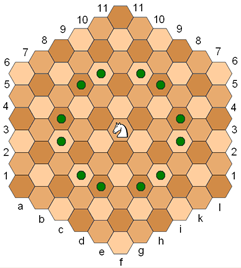
\includegraphics{images/hexKnight.png} & 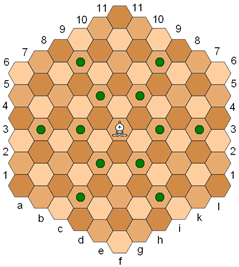
\includegraphics{images/hexBishop.png} \\ \hline 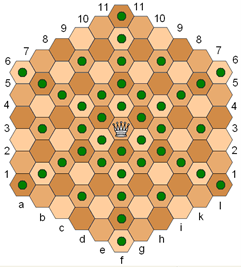
\includegraphics{images/hexQueen.png} & 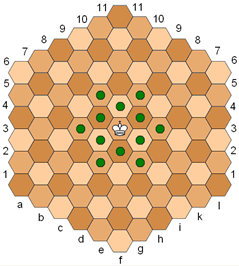
\includegraphics{images/hexKing.png} \\ \hline
    \end{tabular}
    \caption{Gültige Schachzüge in der hexagonalen Variante \protect\footnotemark}
    \label{tab:posMove}
\end{table}
\footnotetext{\url{https://commons.wikimedia.org/wiki/Category:Glinski\%27s_hexagonal_chess}}
\newpage
Der Bauer bleibt weiter die schlechteste Figur des Spiels. Im Vergleich zum normalen Schach gewinnt der Bauer nicht an Zügen und Potential. Am Ende darf der Bauer sich in eine Königin verwandeln. Das macht den Bauern zum Ende des Spiels zu einer wertvollen Figur mit Potential. \cite{GlinskiHexaChess} (vgl. Tabelle \ref{tab:posMove})\par
Der Turm darf sich bis zum Rand in jede Richtung orthogonal bewegen. Spielfiguren behindern seine Bewegungsmöglichkeiten. Der Turm ist die wertvollste Figur nach der Königin. Anders als im normalen Schach ist der Turm allein nicht in der Lage einen König abzuschneiden. Dadurch das der König auch diagonal laufen kann, werden zwei Türme benötigt. Der Turm ist im hexagonalen Schach in der Lage 1/3 des Spielfeldes abzudecken. Im herkömmlichen Schach kann der Turm nur 1/4 von dem Spielfeld abdecken. \cite{GlinskiHexaChess} (vgl. Tabelle \ref{tab:posMove})\par
Das Pferd kann sich auf die Felder bewegen, welche zwei Felder orthogonal entfernt sind und danach jeweils links und rechts oben von der Ausgangsposition. Drei Zügen werden gebraucht, um komplett über das Feld zu kommen. Das Pferd hat sich im Vergleich zum normalen Schach nicht verbessert. \cite{GlinskiHexaChess} (vgl. Tabelle \ref{tab:posMove})\par
Der Bischof bewegt sich diagonal bis zum Ende des Feldes. Der Bischof deckt im hexagonalen Schach 1/7 des Spielfeldes ab. Im normalen Schach wird optimalerweise 1/5 vom Bischof abgedeckt. Drei Bischöfe werden im hexagonalen Schach gebraucht, um den König abzuschneiden. Normalerweise werden dafür nur zwei Bischöfe gebraucht. Im Vergleich der beiden Versionen hat der Bischof an Macht verloren. \cite{GlinskiHexaChess} (vgl. Tabelle \ref{tab:posMove})\par
Die Königin ist weiter die stärkste Figur auf dem Feld. Sie kann sich orthogonal und diagonal bis zum Ende des Feldes bewegen. Dadurch kann die Königin in einem Radius von zwei Feldern alles schlagen. Das ist ein Feld besser als im normalen Schach. Die Königin kann allein den König in Schachmatt stellen, sofern er in eine Ecke gedrängt wird. Ungefähr die Hälfte des Feldes kann die Königin in optimaler Position abdecken. Ein bisschen weniger kann die Königin im normalen Schach abdecken. Weiter noch ist sie nie in der Lage den König allein in ein Schachmatt zu stellen. \cite{GlinskiHexaChess} (vgl. Tabelle \ref{tab:posMove})\par
Der König gewinnt in der Abwandlung an Macht. Er kann sich ein Feld diagonal und orthogonal bewegen. Dadurch werden mehr Türme und Bischöfe gebraucht, um den König auf eine Seite auszugrenzen. Dazu hat der König im hexagonalen Schach vier weitere Bewegungsmöglichkeiten. \cite{GlinskiHexaChess} (vgl. Tabelle \ref{tab:posMove})
